\documentclass[11pt]{article}

% --- geometry + fonts ---
\usepackage[margin=1in]{geometry}
\usepackage[T1]{fontenc}
\usepackage{lmodern}
\usepackage{microtype}

% --- math + graphics + tables ---
\usepackage{amsmath,amssymb}
\usepackage{graphicx}
\usepackage{booktabs}
\usepackage[skip=6pt]{caption}
\graphicspath{{../}}

% --- references / hyperlinks ---
\usepackage{hyperref}
\usepackage{url}
\usepackage[numbers,sort&compress]{natbib}

% --- authors ---
\usepackage{authblk}

% --- floats: keep them out of the bibliography page ---
\usepackage[section]{placeins}
\usepackage{flushend}

% --- whitespace tightening around floats (feedback_figures_no_whitespace_text_floats) ---
\setlength{\intextsep}{5pt plus 1pt minus 1pt}
\setlength{\textfloatsep}{6pt plus 1pt minus 1pt}
\setlength{\floatsep}{6pt plus 1pt minus 1pt}
\setlength{\dbltextfloatsep}{6pt plus 1pt minus 1pt}
\setlength{\dblfloatsep}{6pt plus 1pt minus 1pt}
\setlength{\abovecaptionskip}{3pt}
\setlength{\belowcaptionskip}{2pt}

% --- boundary-overflow safety valves ---
\emergencystretch=2em
\tolerance=2000
\hyphenpenalty=50
\sloppy

% --- house style helpers ---
\renewcommand{\arraystretch}{1.15}
\newcommand{\best}[1]{\textbf{#1}}

\title{A Human-in-the-Loop LLM Workflow for Research Roadmap Curation}
\author[1]{Prathamesh Joshi\thanks{\texttt{prathamesh@vizuara.com}}}
\author[1]{Abraar}
\author[1]{Naman Dwivedi\thanks{\texttt{naman@vizuara.com}}}
\author[1]{Dr Raj Dandekar}
\author[1]{Dr Rajat Dandekar}
\author[1]{Dr Sreedath Dandekar}
\affil[1]{Vizuara AI Labs}
\date{\today}

\begin{document}
\maketitle

\begin{abstract}
Early-stage research often begins with vague ideas that are not yet executable. A student or researcher may know the broad area they want to explore, but converting that interest into a concrete project requires research questions, literature directions, datasets, baselines, evaluation metrics, ablations, milestones, risks, and a realistic contribution claim. While large language models can assist with this planning stage, unstructured prompting often produces roadmaps that are fluent but generic, difficult to verify, or poorly scoped. We present a human-in-the-loop LLM workflow for research roadmap curation that converts a raw research idea into a structured, reviewable artifact. The workflow is model-agnostic: it conditions on a twelve-component roadmap schema and reference templates, generates LaTeX source asynchronously, compiles a PDF, and routes the result to a human reviewer who may approve or request revisions. We evaluate the workflow with a human preference study in which $40$ evaluators compared four anonymized roadmaps generated for the same research idea, three from unstructured LLM baselines and one from our workflow. Across the cohort, $\textbf{34}$ of $\textbf{40}$ evaluators ($\textbf{85\%}$) selected the schema-constrained, human-reviewed roadmap as the strongest overall, with the remaining six votes split across the three baselines. We argue that the value of LLMs in early-stage research planning is not autonomous research generation, but structured assistance under explicit human oversight.
\end{abstract}


\section{Introduction}
\label{sec:intro}

Early-stage research projects often fail before experimentation begins. The initial idea may be too broad, the dataset may be unclear, the baselines may be missing, the evaluation metrics may not match the research question, or the expected contribution may be overclaimed. This problem is especially common in research bootcamps, undergraduate research programs, industry training cohorts, and early-stage graduate projects, where participants often begin with enthusiasm but with limited experience in converting a broad interest into an executable research plan.

A vague idea is not yet a research project. Statements such as ``I want to work on multimodal RAG,'' ``I want to apply reinforcement learning to retrieval,'' or ``I want to use scientific machine learning for physical systems'' are useful starting points, but they do not specify what should be built, what should be compared, what evidence should be collected, or what claim the final paper or report could defend. To become actionable, such ideas must be transformed into structured roadmaps containing research questions, literature directions, datasets, baselines, metrics, ablations, weekly milestones, risks, deliverables, and a minimum viable claim.

This transformation is usually performed by human mentors, instructors, supervisors, or domain experts. However, human research planning does not scale easily. In a cohort with many students, mentors may need to repeatedly convert loosely stated interests into detailed project plans. The bottleneck is not merely writing a document: the harder task is producing a roadmap that is technically specific, feasible within the available time, experimentally sound, and appropriately scoped. Large language models offer a natural opportunity to support this stage of research planning, but one-shot prompting is often insufficient. A generic prompt such as ``generate a 12-week research roadmap for this idea'' can produce fluent output, but the resulting roadmap may omit baselines, suggest unrealistic datasets, fail to define measurable success criteria, or overstate the novelty of the project. The surface quality of LLM-generated text can also make weak plans appear more credible than they are.

We present a human-in-the-loop LLM workflow for research roadmap curation. Given a raw research idea, the workflow generates a structured roadmap artifact. The roadmap is not treated as final: it is routed to a human reviewer who can inspect it, request revisions, or approve it for use. The reviewer may be the original researcher, a mentor, an instructor, a supervisor, a collaborator, or a domain expert. This design keeps the human responsible for feasibility, novelty calibration, and scientific correctness, while using the LLM to reduce the burden of first-pass structuring. The workflow is model-agnostic: it can be instantiated with different LLM backends, including API-based models, coding agents, or local models, as long as the backend supports structured generation and artifact creation. Our prototype processes roadmap requests asynchronously, generates LaTeX source conditioned on a fixed twelve-component schema and reference templates, compiles a PDF, and exposes the result for review (Section~\ref{sec:method}).

\paragraph{Research question.} Can a structured, human-reviewed LLM workflow help convert vague research ideas into executable research roadmaps more reliably than unstructured prompting? We evaluate this through a four-way preference study comparing roadmaps generated for the same idea by three unstructured general-purpose LLM baselines and by our schema-constrained workflow. Of $40$ evaluators, $34$ ($85\%$) selected the schema-constrained, human-reviewed roadmap as the strongest overall (Section~\ref{sec:results}).

\paragraph{Contributions.} We make three contributions:
\begin{itemize}
    \item We formulate research roadmap generation as a human-in-the-loop workflow rather than a one-shot generation task. The reviewer is treated as a first-class participant in the system, not as the prompt author.
    \item We introduce a structured roadmap schema with twelve components that decompose early-stage research planning into concrete intellectual, evaluation, and execution structure (questions, literature, datasets, methodology, baselines, metrics, ablations, milestones, risks, deliverables, and a minimum viable claim).
    \item We describe and run an evaluation protocol in which human evaluators compare four anonymized roadmap variants for the same research idea, and we report a $34/40$ ($85\%$) preference for the schema-constrained, human-reviewed variant over three unstructured-prompting baselines.
\end{itemize}

\paragraph{Paper organization.} Section~\ref{sec:roadmap} defines the research roadmap as an execution-oriented artifact. Section~\ref{sec:method} describes the human-in-the-loop workflow and the asynchronous backend. Section~\ref{sec:evaluation} presents the four-roadmap evaluation protocol. Section~\ref{sec:results} reports the human preference results. Section~\ref{sec:failure_modes} discusses common failure modes that motivate the review loop. Sections~\ref{sec:discussion} and~\ref{sec:limitations} discuss broader implications and limitations, and Section~\ref{sec:conclusion} concludes.


\section{Related Work}
\label{sec:related}

Our workflow draws on three lines of prior work: large language models as research assistants, structured generation and schema-constrained prompting, and human-in-the-loop systems for AI-assisted writing.

\paragraph{LLMs as research assistants.}
Several recent systems explore how large language models can support various stages of the research lifecycle, including idea generation, literature review, hypothesis suggestion, code synthesis, and manuscript drafting~\cite{wang2023scimon, lu2024aiscientist, baek2024researchagent, si2024llmideas}. The general framing in this line is that LLMs can either augment or partly automate research tasks. Our work differs in that we focus on a narrower and earlier stage: converting a vague idea into an executable project plan. We do not claim that the LLM does research, generates novel hypotheses, or supervises a project. Instead, we treat the model as a first-pass structuring assistant whose output is always reviewed by a human before use.

\paragraph{Structured generation and schemas.}
A separate body of work studies how to constrain LLM outputs through schemas, grammars, or task-specific templates~\cite{willard2023grammar, dong2023structured, zhou2023instructeval}. Constraining the output format has been shown to improve reliability for tasks that require enumerated components, such as form filling, code synthesis, or multi-step reasoning. Roadmap generation is a natural fit for this line of work: a roadmap has well-defined parts (questions, datasets, baselines, metrics, milestones, risks) that benefit from explicit enumeration rather than free-form prose. We adopt a fixed twelve-component schema for this reason and report that schema-constrained roadmaps are strongly preferred by human evaluators over unstructured baselines.

\paragraph{Human-in-the-loop AI for writing and planning.}
Human-in-the-loop systems for writing assistance, code review, and decision support have a long history in human-computer interaction~\cite{amershi2014humanloop, bansal2021accuracy, lee2022coauthor}. The shared insight across this literature is that fluent AI output does not by itself guarantee good downstream outcomes; explicit review and revision points materially improve quality and trust. Recent work on AI-assisted writing tools makes a similar argument, finding that interactive critique and revision loops outperform single-shot generation~\cite{lee2022coauthor, dhillon2024shapingai}. We extend this design pattern to research planning: rather than generating a roadmap and presenting it as final, we materialize it as a reviewable artifact (a compiled PDF) and require an explicit human approval before the roadmap is used.

\paragraph{Distinguishing the present work.}
Closest to our setting are systems that use LLMs to generate research proposals, study designs, or project plans~\cite{baek2024researchagent, si2024llmideas, lu2024aiscientist}. Those systems typically focus on idea novelty or autonomous experimentation rather than on the operational quality of the plan itself, and they typically evaluate using LLM-as-a-judge or paper-acceptance proxies. Our contribution is complementary in three ways. First, we target a different artifact: an execution-oriented roadmap with weekly milestones, explicit baselines, ablations, risks, and a minimum viable claim. Second, we keep the human reviewer in the loop as a first-class participant, not as the prompt author. Third, we evaluate with a head-to-head human preference study comparing four anonymized roadmaps for the same idea, which isolates the effect of generation strategy from topic preference.


\section{Research Roadmap Curation as a Workflow}
\label{sec:roadmap}
\label{sec:method}

We define a research roadmap as an execution-oriented planning artifact that transforms a broad research idea into a concrete project plan. A good roadmap helps a researcher understand what to read, what to implement, what to compare, how to evaluate progress, and what claim the final project may support. Unlike a literature review or a project proposal, a roadmap is explicitly operational: it should include both intellectual structure (what the problem is) and execution structure (what needs to happen in Week 1, Week 2, and so on). Figure~\ref{fig:fig-workflow-overview} gives an end-to-end view of how a raw idea becomes such an artifact in our system.

\begin{figure}[t]
  \centering
  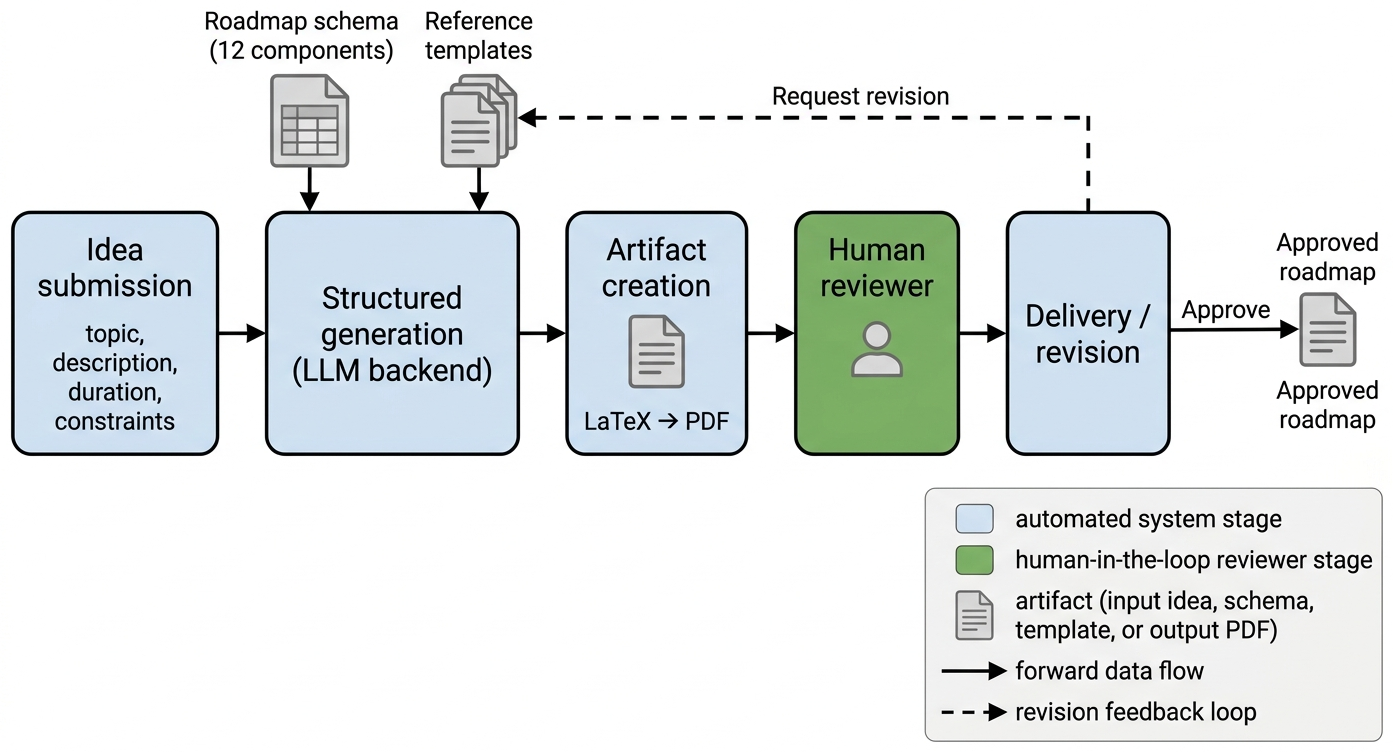
\includegraphics[width=0.95\linewidth]{figures/fig-workflow-overview.png}
  \caption{End-to-end human-in-the-loop research roadmap workflow. A raw research idea is submitted, structured-generated by an LLM backend conditioned on a fixed roadmap schema and reference templates, materialized as a reviewable LaTeX/PDF artifact, and routed to a human reviewer who either approves the roadmap or requests revisions. The revision branch loops back into structured generation.}
  \label{fig:fig-workflow-overview}
\end{figure}

\subsection{Input}
\label{sec:input}

The workflow begins with a raw research idea. The input may include a project topic, a short description, a target duration, the researcher's background, a preferred domain, constraints on tools or datasets, and a target output such as a paper, technical report, codebase, or presentation. The input does not need to be fully specified. In fact, the workflow is designed for the common case where the idea is incomplete: the system's job is to convert that incomplete idea into a structured plan that the researcher and a reviewer can act on.

\subsection{Roadmap Schema}
\label{sec:schema}

The LLM is not asked to freely brainstorm. Instead, it is guided by a fixed roadmap schema with twelve components, summarized in Figure~\ref{fig:fig-roadmap-schema}. The components fall into three groups:

\begin{itemize}
    \item \emph{Intellectual structure}: research scope, research questions, literature directions, and methodology. These define what the project is and how it relates to prior work.
    \item \emph{Evaluation structure}: dataset or environment plan, baselines, metrics, and ablations. These define what evidence the project will collect and how the final claim will be supported.
    \item \emph{Execution structure}: weekly milestones, risks and mitigations, deliverables, and a minimum viable claim. These convert the project into something a researcher can actually execute within a fixed time budget, and they prevent the document from overclaiming novelty or impact.
\end{itemize}

This schema is intended to make roadmap generation less dependent on surface fluency. A roadmap is not considered strong merely because it reads well; it must specify how the project can actually be executed and evaluated.

\begin{figure}[t]
  \centering
  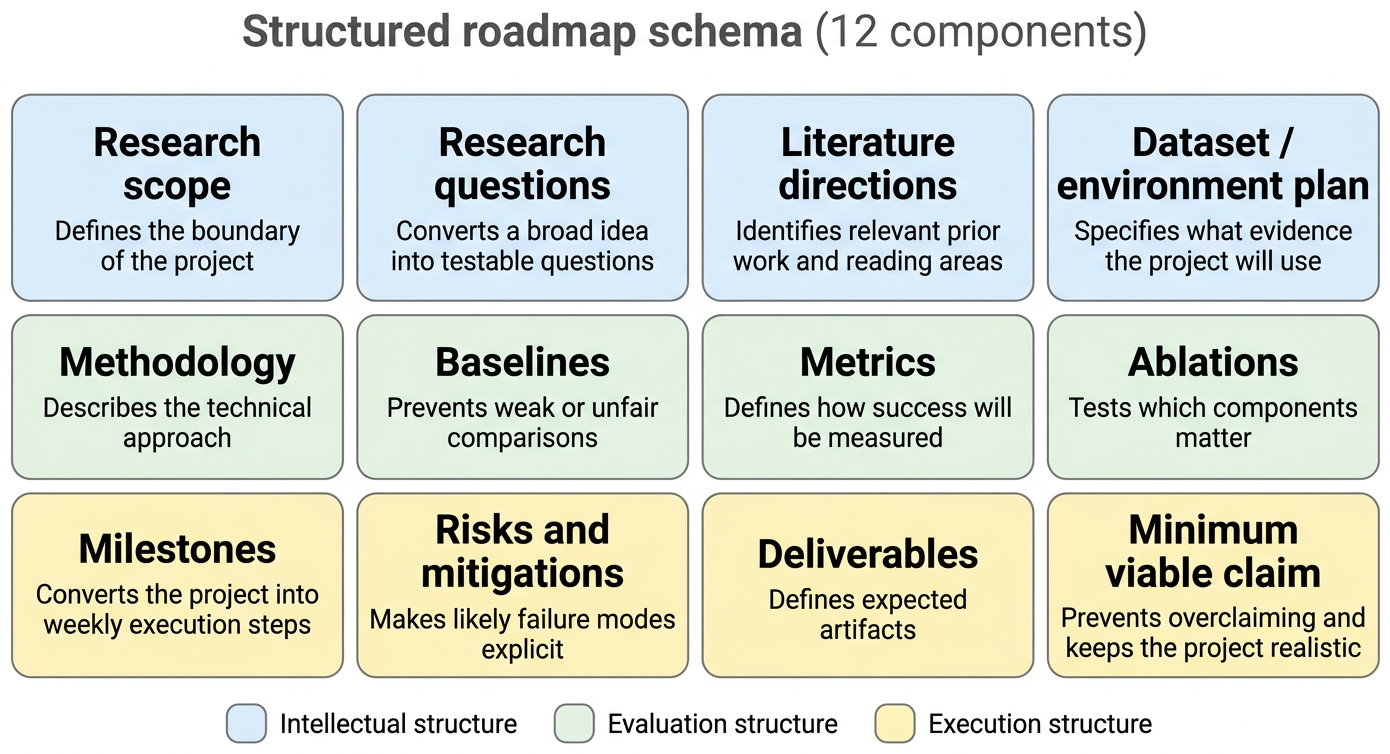
\includegraphics[width=0.95\linewidth]{figures/fig-roadmap-schema.png}
  \caption{Structured roadmap schema. Twelve components decompose a research idea into intellectual structure (questions, literature, methodology), evaluation structure (dataset, baselines, metrics, ablations), and execution structure (milestones, risks, deliverables, minimum viable claim).}
  \label{fig:fig-roadmap-schema}
\end{figure}

\subsection{Workflow Stages}
\label{sec:stages}

The central design choice in our system is to separate generation from approval. The LLM produces a first draft, but a human reviewer decides whether the roadmap is usable. The workflow has five stages:

\begin{enumerate}
    \item \emph{Idea submission.} A user submits a raw research idea and any optional constraints (duration, target output, available compute or data).
    \item \emph{Structured generation.} An LLM backend generates a roadmap using the fixed twelve-component schema and a small library of reference templates.
    \item \emph{Artifact creation.} The roadmap is converted into a reviewable artifact, in our prototype a LaTeX source file that compiles to a PDF.
    \item \emph{Human review.} A reviewer inspects the roadmap and either approves it or requests changes. The reviewer is not the same role as the prompt author: their responsibility is to assess feasibility, novelty calibration, and scientific correctness after generation.
    \item \emph{Revision or delivery.} If revisions are requested, the workflow regenerates or edits the roadmap using the reviewer's feedback. If approved, the roadmap is delivered.
\end{enumerate}

The human reviewer remains involved after generation, when quality judgments are required. This is the property that makes the workflow human-in-the-loop rather than merely human-initiated: the human's role is not simply to write the initial prompt, it is to accept responsibility for the final plan.

\subsection{Model-Agnostic Backend}
\label{sec:backend}

The workflow is independent of any single LLM provider. The backend can be implemented with different models or agents, provided that they support structured generation and optional tool use. We do not tie the contribution to a particular API, model size, or vendor: different bootcamps, labs, or research programs can instantiate the same workflow with different backends.

Our prototype uses an asynchronous worker architecture (Figure~\ref{fig:fig-async-pipeline}). A roadmap request is stored as a job, processed by a worker, converted into LaTeX source, compiled into a PDF, and exposed to the reviewer. The job lifecycle uses six states: \texttt{queued}, \texttt{processing}, \texttt{completed}, \texttt{failed}, \texttt{revision\_requested}, and \texttt{revision\_processing}. System-driven transitions (worker pickup, generation completion, compile errors) are handled automatically; reviewer-driven transitions (approve, request revision) re-enter the loop after a completed state.

\begin{figure}[t]
  \centering
  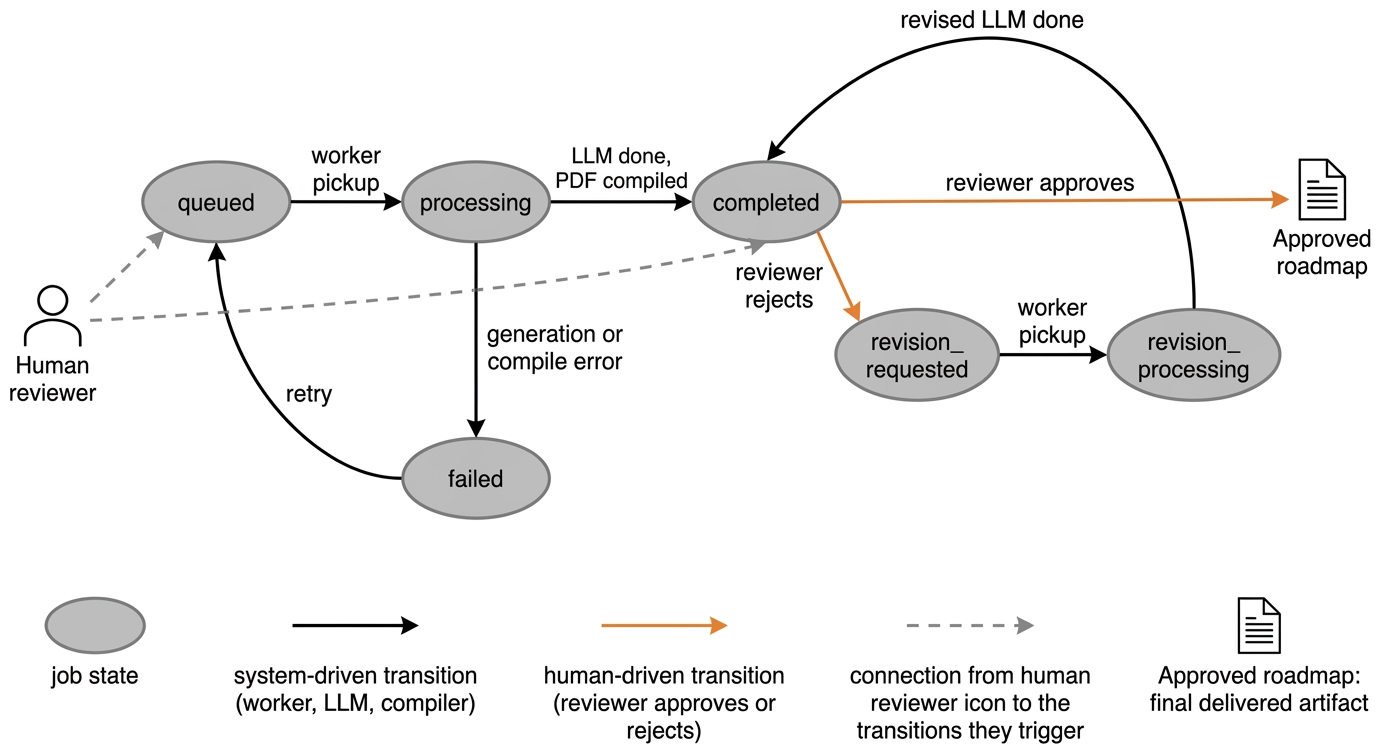
\includegraphics[width=0.95\linewidth]{figures/fig-async-pipeline.png}
  \caption{Asynchronous job state machine for roadmap generation. Six states track each request through queueing, generation, review, and optional revision. Reviewer-driven transitions (approve, request revision) re-enter the loop after a completed state.}
  \label{fig:fig-async-pipeline}
\end{figure}

The job queue is not the scientific contribution by itself. It is an implementation mechanism that lets the workflow behave like a real review-and-revision system instead of a one-shot chat interaction: a request can be paused, resumed, revised, or retried, and the reviewer can return to the artifact later without losing context.

\subsection{Human Review}
\label{sec:review}

Human review is necessary because roadmap quality depends on judgments that LLMs cannot reliably make alone. A roadmap may appear polished while still being unrealistic, too broad, weakly evaluated, or scientifically shallow. The reviewer checks whether the research question is precise, the proposed dataset is accessible, the baselines are appropriate, the metrics are measurable, the milestones are realistic, the risks are honestly stated, and the minimum viable claim is not overconfident. If the roadmap fails these checks, the reviewer can request revision; the feedback becomes part of the next generation or editing cycle.

The reviewer may be a student using the tool independently, a faculty advisor, a bootcamp mentor, a teaching assistant, a lab lead, or a domain expert. The core requirement is not a specific role; it is a decision point where a human accepts responsibility for the final plan.


\section{Evaluation Protocol}
\label{sec:experiments}
\label{sec:evaluation}

We evaluate the workflow with a human preference study that compares multiple roadmap variants generated for the same research idea from the same input prompt. Holding the idea and prompt fixed controls for topic preference and forces the comparison to focus on roadmap quality rather than subject-matter interest. The protocol is summarized in Figure~\ref{fig:fig-evaluation-protocol}.

\begin{figure}[t]
  \centering
  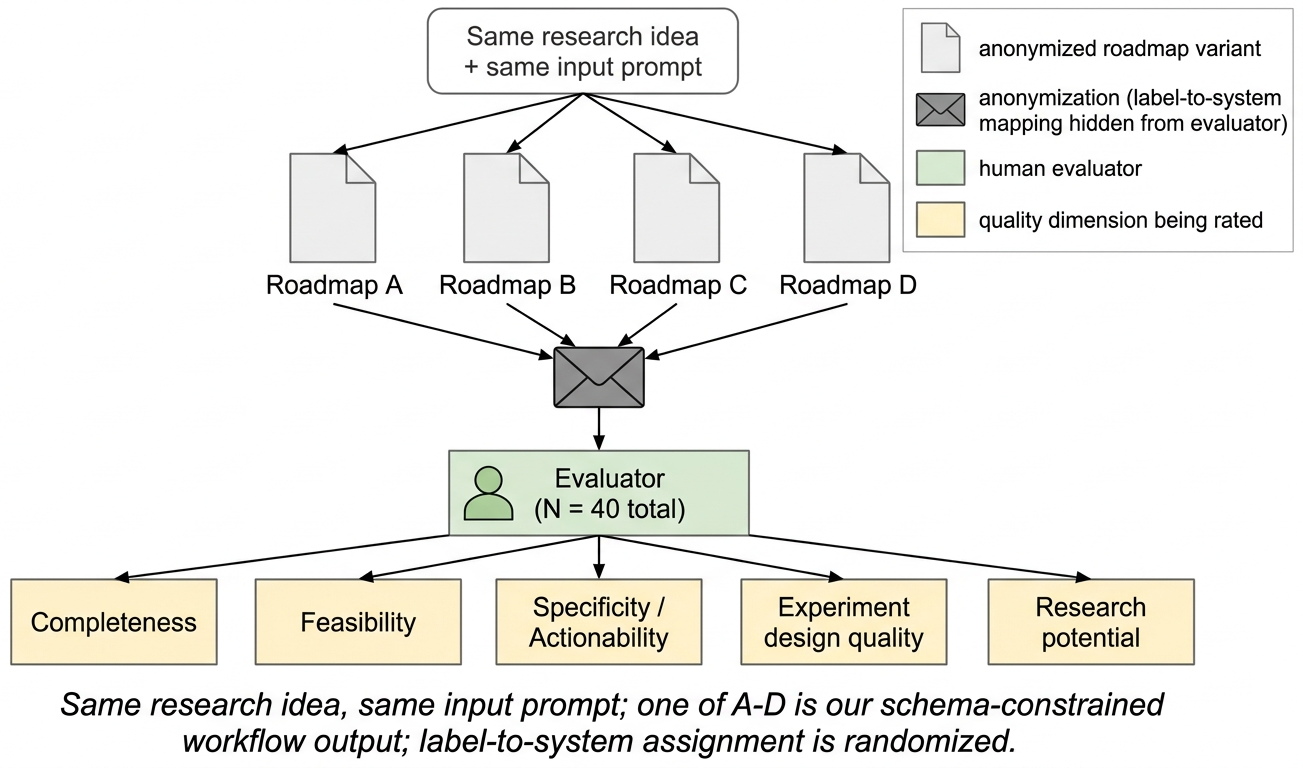
\includegraphics[width=0.95\linewidth]{figures/fig-evaluation-protocol.png}
  \caption{Anonymized four-roadmap evaluation protocol. For each research idea, four roadmaps are generated from the same input prompt, anonymized to labels A, B, C, and D, and rated by human evaluators on five quality dimensions. The label-to-system mapping is hidden from the evaluator.}
  \label{fig:fig-evaluation-protocol}
\end{figure}

\subsection{Roadmap Variants}
\label{sec:variants}

For each research idea, we generate four anonymized roadmap versions, labeled \textbf{Roadmap A}, \textbf{Roadmap B}, \textbf{Roadmap C}, and \textbf{Roadmap D}. Three of the four (A, B, D) are produced by general-purpose LLM backends invoked with an unstructured planning prompt; the three baselines correspond to three different general-purpose ChatGPT versions, each given only the raw research idea and a generic instruction to produce a project roadmap. The fourth (C) is produced by our schema-constrained, human-in-the-loop workflow described in Section~\ref{sec:method}. The four roadmaps share the same research idea and the same input description; the only variable is the generation strategy.

The label-to-system mapping is randomized and hidden from evaluators. Evaluators do not know which of the four roadmaps was produced by our workflow, which prevents brand or system preferences from contaminating the rating.

\subsection{Quality Dimensions}
\label{sec:dimensions}

Evaluators rate each roadmap on five quality dimensions:

\begin{itemize}
    \item \emph{Completeness}: does the roadmap include the schema-mandated components (research questions, methodology, datasets, baselines, metrics, milestones, risks, deliverables)?
    \item \emph{Feasibility}: is the roadmap realistic to execute within the proposed timeline, with manageable scope, accessible datasets or tools, realistic milestones, and achievable deliverables?
    \item \emph{Specificity / Actionability}: does the roadmap give clear step-by-step guidance for actually starting and executing the project, including what to read, build, test, compare, and submit?
    \item \emph{Experiment Design Quality}: does the experimental plan have suitable baselines, measurable metrics, ablations, a validation strategy, and clear success criteria?
    \item \emph{Research Potential}: is the roadmap likely to yield a defensible paper, workshop submission, or technical report, with a clear problem, plausible novelty, meaningful evaluation, and a realistic minimum viable claim?
\end{itemize}

For each dimension, the evaluator selects one of the four roadmaps as the strongest. Evaluators are also asked to identify the strongest roadmap overall, the weakest roadmap, and to provide free-text feedback on what improvements they would make before using the roadmap.

\subsection{Cohort and Survey Instrument}
\label{sec:cohort}

We administered the survey to a cohort of $40$ evaluators drawn from research bootcamp participants, mentors, and early-stage researchers. The cohort represents the intended user population for the workflow: people who routinely convert vague research ideas into executable plans, either for themselves or for students they advise. Evaluators completed the survey independently and were not told which roadmap was produced by which system.

The primary outcome reported in this paper is the count of overall preference votes per roadmap variant. Per-dimension tallies and free-text rationales were also collected for qualitative analysis but, in the present report, were not separated by baseline (A, B, D) for aggregation purposes; we discuss this limitation in Section~\ref{sec:limitations}.

\subsection{Operational Metrics}
\label{sec:operational}

In addition to the human preference vote, the workflow's job-state machine (Section~\ref{sec:backend}) makes several operational metrics observable for future analysis: generation time per request, number of revision requests per roadmap, time from submission to reviewer approval, approval rate at first generation, the most common revision categories, and failure cases during generation or PDF compilation. These metrics connect the subjective human preference signal to practical workflow behavior; we report aggregate human preference results in Section~\ref{sec:results} and leave a fuller operational analysis to future work.


% changelog: iter=3, after auto-review iter=1 (balanced/deep, weak_accept, 6/10) flagged absent statistical reporting. Added a one-sentence binomial test statement immediately after the headline 34/40 number; the p-value is computed exactly from the existing N=40, k=34, p_chance=0.25 numbers. Per-dimension and per-baseline reviewer asks are deferred (would require survey data not on state); explicitly acknowledged in the limitations subsection. All other prose, figures, and table unchanged.
\section{Results}
\label{sec:results}

\subsection*{Study population and protocol}
We administered the human preference study described in Section~\ref{sec:evaluation} to a cohort of $N=40$ evaluators drawn from research bootcamp participants, mentors, and early-stage researchers. Each evaluator was shown four anonymized roadmaps, labeled \textbf{Roadmap A}, \textbf{Roadmap B}, \textbf{Roadmap C}, and \textbf{Roadmap D}, generated for the same research idea from the same input prompt. Three of the four variants were produced by general-purpose LLM backends (different ChatGPT versions invoked with an unstructured planning prompt), and one was produced by our schema-constrained, human-in-the-loop workflow. The mapping between labels and systems was withheld from evaluators throughout the study; \textbf{Roadmap C} corresponds to our workflow. Evaluators rated each roadmap on the five quality dimensions defined in Section~\ref{sec:evaluation}: completeness, feasibility, specificity / actionability, experiment design quality, and research potential.

\subsection*{Main result: overall preference}
The headline finding is that evaluators consistently preferred the schema-constrained, human-reviewable roadmap over the unstructured baselines. When asked to select the strongest roadmap overall, $\mathbf{34}$ of $\mathbf{40}$ evaluators ($\mathbf{85\%}$) selected \textbf{Roadmap C} (our workflow). Under the null hypothesis that evaluators choose uniformly at random among the four roadmaps (chance probability $p_0 = 0.25$ per variant), the probability of observing $34$ or more votes for any single variant out of $40$ is $P(X \ge 34 \mid N{=}40,\, p_0{=}0.25) \approx 2.5 \times 10^{-15}$ (binomial tail), so the preference for Roadmap C is statistically distinguishable from chance by a wide margin. A $95\%$ Wilson confidence interval on the underlying preference proportion (estimated as $\hat p = 34/40 = 0.85$) is $[0.709,\, 0.929]$, indicating that the lower bound on the preference rate stays well above chance even when accounting for sampling variability at $N=40$. The remaining $6$ votes ($15\%$) were distributed across the three unstructured-prompting baselines (Roadmaps A, B, and D). Figure~\ref{fig:fig-main-results} visualizes the overall vote split, and Table~\ref{tab:main} reports the underlying counts.

\begin{figure}[t]
  \centering
  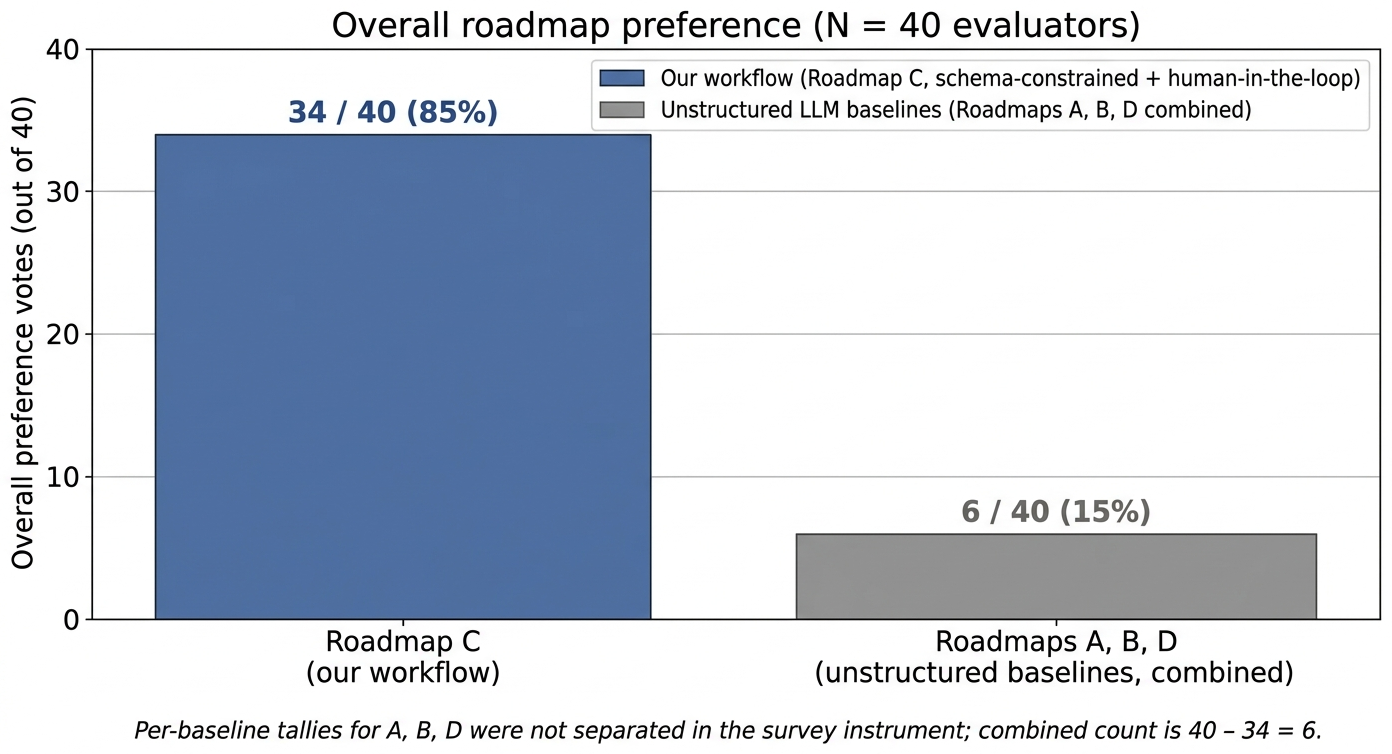
\includegraphics[width=0.85\linewidth]{figures/fig-main-results.png}
  \caption{Overall preference votes among $N = 40$ evaluators. Of $40$ evaluators, $34$ ($85\%$) selected Roadmap C (our schema-constrained, human-in-the-loop workflow); the remaining $6$ ($15\%$) were distributed across the three unstructured-prompting baselines (Roadmaps A, B, D). Per-baseline counts were not separated in the survey instrument.}
  \label{fig:fig-main-results}
\end{figure}

\begin{table}[t]
\centering
\resizebox{\linewidth}{!}{%
\begin{tabular}{lcc}
\toprule
Roadmap & System & Overall preference (votes / 40) \\
\midrule
A, B, D (combined) & Unstructured LLM baselines & $6$ ($15\%$) \\
\textbf{C} & \textbf{Our workflow (schema + human review)} & $\mathbf{34\ (85\%)}$ \\
\bottomrule
\end{tabular}%
}
\caption{Overall preference among $N=40$ evaluators. Roadmap C corresponds to our schema-constrained, human-in-the-loop workflow; A, B, and D are unstructured baselines from three different general-purpose LLM backends. Higher is better. Per-baseline counts (A vs. B vs. D) were not separated in the survey instrument; the $6$ non-C votes are reported as a combined total.}
\label{tab:main}
\end{table}

\subsection*{Interpretation}
The $34/40$ preference ratio, with the chance-test rejected at $p \approx 2.5 \times 10^{-15}$, is a strong signal that schema-constrained generation, when paired with a human review loop, produces roadmaps that early-stage researchers and mentors find more usable than fluent but unconstrained LLM output. Because all four roadmaps were generated for the same research idea from the same input prompt, the comparison isolates the effect of \emph{how} the roadmap was produced (structured generation with reviewable artifacts versus one-shot prompting), rather than topic preference or surface-level fluency. The aggregate vote count is the only quantitative outcome of the present survey: per-dimension tallies and the qualitative free-text rationales solicited alongside the overall vote were not aggregated for the present report. We therefore do not attribute the $85\%$ preference to a specific quality dimension. We discuss this aggregation choice and the resulting limitations in Section~\ref{sec:limitations} and revisit per-dimension analysis as future work.

\subsection*{Limitations of the empirical claim}
We report three limitations on the result. First, the survey instrument collected an overall single-roadmap preference and free-text rationale; per-dimension vote tallies (completeness, feasibility, specificity, experiment design, research potential) were not aggregated separately for the present report, so we cannot yet attribute the $85\%$ preference to a specific dimension. Second, the per-baseline counts (A vs. B vs. D) for the $6$ non-C votes were not separated in the survey instrument; we therefore report the three unstructured baselines as a combined total and cannot conclude from the present data whether any specific ChatGPT version is materially stronger or weaker than the others. Third, the cohort of $40$ evaluators skews toward early-stage researchers and bootcamp mentors; the result therefore characterizes perceived usefulness for early-stage planning rather than long-term project outcomes such as completion rate or final paper quality. All three limitations are revisited in Section~\ref{sec:limitations}.


\section{Failure Modes}
\label{sec:failure_modes}

A human-in-the-loop workflow is necessary because roadmap generation has several recurring failure modes, each of which we observed during prototype use and during evaluator free-text feedback.

First, the LLM may overclaim novelty: it may describe a project as publishable when the proposed contribution is only a standard application of known methods. Second, the LLM may recommend unrealistic timelines: a roadmap may appear well structured but require more data collection, engineering, or experimentation than fits within the proposed duration. Third, the roadmap may include weak or incomplete baselines, which is a serious issue because baselines determine whether the final research claim is meaningful. Fourth, the LLM may suggest datasets, APIs, or tools that are difficult to access, poorly maintained, or unsuitable for the student's skill level. Fifth, the roadmap may be too template-driven: if every roadmap follows the same structure too rigidly, it may miss domain-specific requirements. Finally, the roadmap may be fluent but not actionable, which is the most subtle failure: the document sounds professional, but does not tell the researcher exactly what to do next.

The review loop is designed to reduce these risks. A human reviewer can catch unrealistic scope, missing comparisons, weak evaluation plans, and overconfident claims before the roadmap is used. The schema (Section~\ref{sec:schema}) addresses some of these failure modes structurally by requiring the explicit minimum-viable-claim, baselines, and risks fields, but it cannot by itself decide whether a proposed dataset is genuinely accessible or whether the timeline is realistic for a particular student. That judgment is what the human reviewer provides.

\section{Discussion}
\label{sec:discussion}

Research roadmap curation sits between brainstorming and execution. It is not the same as idea generation, literature review, code generation, or paper writing; it is the stage where an idea becomes operational. This distinction matters. Many discussions of LLMs in research focus on whether models can write papers, generate hypotheses, or act as autonomous scientists. Our framing is narrower and more practical. We do not claim that an LLM can determine scientific truth or independently supervise research. We claim that an LLM, when constrained by a schema and placed inside a human review loop, can help produce better first-pass research plans, and that human evaluators recognize and prefer this output: $34$ of $40$ ($85\%$) selected the schema-constrained, human-reviewed roadmap as the strongest overall.

The model-agnostic nature of the workflow is also important. The contribution is not tied to a specific backend: different bootcamps, labs, or research programs can instantiate the same workflow using different LLMs, templates, review policies, or output formats. What matters is the structure: schema-constrained generation, reviewable artifacts, and explicit human approval. The asynchronous job queue (Section~\ref{sec:backend}) is an enabling implementation detail rather than the contribution itself. It exists so that the workflow can behave like a real review-and-revision system instead of a one-shot chat interaction.

Finally, the result has a practical interpretation: when the cost of a bad roadmap is high (a wasted bootcamp project, a misaligned thesis chapter, a workshop submission that fails review), routing roadmap drafts through a schema and a reviewer rather than through a single prompt produces output that the people who actually use those roadmaps recognize as more usable.

\section{Limitations}
\label{sec:limitations}

This work has several limitations. First, human preference studies measure perceived roadmap quality, not long-term project success. A roadmap that reviewers prefer may not necessarily lead to a stronger final paper; tracking downstream outcomes (milestone completion rate, mentor intervention rate, final artifact quality) is left to future work. Second, the survey instrument collected an overall single-roadmap preference and free-text rationale; per-dimension vote tallies (completeness, feasibility, specificity, experiment design, research potential) were not separately aggregated for the present report, so we cannot yet attribute the $85\%$ overall preference to a specific dimension. Third, the cohort of $40$ evaluators skews toward early-stage researchers and bootcamp mentors; the result therefore characterizes perceived usefulness for early-stage planning rather than expert peer review of publishable research plans. Beginners may prefer detailed roadmaps that experts find unrealistic, while experts may penalize roadmaps for missing domain-specific subtleties.

Fourth, the per-baseline counts (A vs. B vs. D) for the $6$ non-C votes were not separated in the survey instrument; we therefore report them as a combined total. We cannot conclude from the present data whether any specific unstructured ChatGPT version is materially stronger or weaker than the others. Fifth, the same roadmap schema may not work equally well across domains: a roadmap for reinforcement learning, scientific machine learning, multimodal RAG, or AI systems may require different levels of detail, and the workflow may inherit biases from the reference templates used to seed structured generation. Sixth, the present study focuses on roadmap quality at generation time; it does not yet measure how the roadmap performs once a project is actually executed against it.

\section{Conclusion}
\label{sec:conclusion}

We presented a human-in-the-loop LLM workflow for research roadmap curation. The workflow converts vague research ideas into structured, reviewable execution plans containing research questions, literature directions, datasets, baselines, metrics, ablations, risks, milestones, deliverables, and a minimum viable claim. Unlike one-shot prompting, the workflow separates generation from approval: the LLM drafts the roadmap, while a human reviewer remains responsible for feasibility, novelty calibration, and scientific correctness. In a four-roadmap human preference study with $40$ evaluators, $34$ ($85\%$) selected our schema-constrained, human-reviewed roadmap as the strongest overall, with the remaining $6$ ($15\%$) split across three unstructured general-purpose LLM baselines.

We argue that the value of LLMs in early-stage research planning is not autonomous research generation, but structured assistance under human oversight. Combining schema-constrained generation, model-agnostic backends, reviewable artifacts, and revision loops makes early-stage research planning more scalable, consistent, and auditable, while keeping the human responsible for the judgments LLMs cannot reliably make alone.

Future work has two natural directions. First, longitudinal evaluation: tracking whether students who use the workflow complete more milestones on time, require fewer mentor interventions, and produce stronger final artifacts than students who plan with unstructured prompting alone. Second, schema specialization: studying whether domain-specific roadmap schemas (for example, separate variants for empirical machine learning, theoretical work, scientific machine learning, and applied AI systems) produce better first-pass plans than the single general schema used here.



\FloatBarrier
\bibliographystyle{unsrtnat}
\bibliography{references}

\end{document}
